\chapter{Program Execution}

\section{Searching for the Program and Block for Machining \\ the Workpiece (PROGRAM/BLOCK SEARCH)}

To execute a program, the program to be run must be an \textbf{active program}.  
It must be displayed on \textbf{line 1} of the screen and positioned at the top of the program number list in the main program memory.

\subsection{Searching for the Program for Machining the Workpiece}

\begin{itemize}
    \iconitem{Press the \textbf{MANUAL} key.}{manual.jpg}
\end{itemize}

\vspace{.5cm}

\begin{itemize}
    \iconitem{Press the \textbf{MENU} key.}{menu.jpg}
\end{itemize}

\vspace{.5cm}

The screen displays the main menu of the command sub-modes:

\begin{center}
    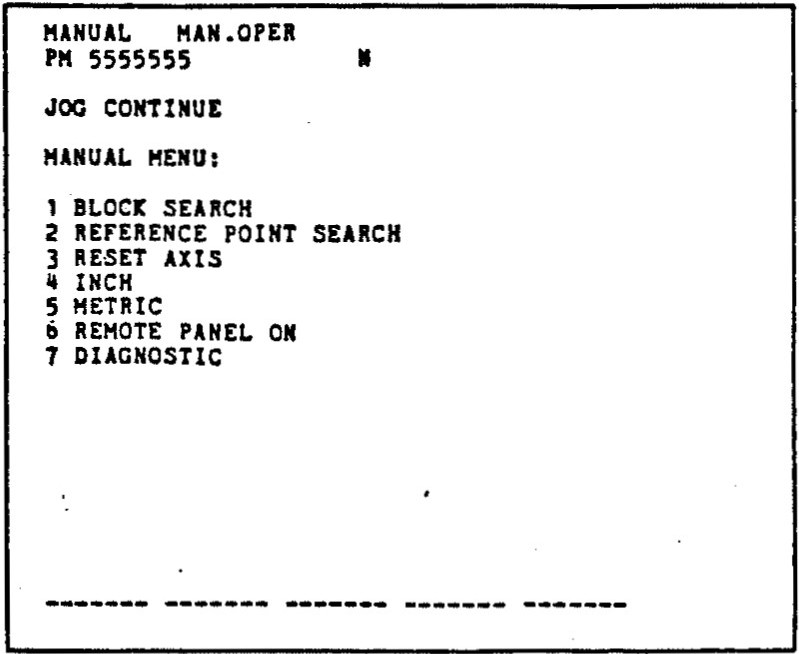
\includegraphics[width=0.7\textwidth]{manual_menu.jpg}
\end{center}

\vspace{.5cm}

Enter the number \textbf{1 (BLOCK SEARCH)} using the numeric keypad.

The active main program currently in progress appears on the screen.

\newpage

\begin{itemize}
    \iconitem{Press the \textbf{F3} function key (ID-DIR).}{f3.jpg}
\end{itemize}

The screen displays the list of program numbers stored in the main program memory.

The indication \textbf{N-SEARCH} (search for the program or block for machining the workpiece) appears on \textbf{line 1} of the screen.

\textbf{Two search possibilities exist:}

\vspace{.5cm}

\textbf{First Search Option:}

\begin{itemize}
    \iconitem{Move the cursor to the line containing the program number \textbf{N} using the \textbf{"up-down"} command keys.}{up.jpg,down.jpg}
\end{itemize}

\begin{itemize}
    \iconitem{Press the \textbf{SEARCH} key to start the search process.}{search.jpg}
\end{itemize}

\vspace{.5cm}

\textbf{Second Search Option:}

\begin{itemize}
    \item Enter the program number \textbf{N} to be searched using the numeric keypad.
\end{itemize}

\begin{itemize}
    \iconitem{Press the \textbf{ENTER} key.}{enter.jpg}
\end{itemize}

The entered program number \textbf{N} appears on \textbf{line 21} of the screen.

\begin{itemize}
    \iconitem{Press the \textbf{SEARCH} key to start the search process.}{search.jpg}
\end{itemize}

\vspace{.5cm}

The search process runs while the \textbf{BUSY} indication is displayed on \textbf{line 1} of the screen.  
Once the search process is completed, the first blocks of the found program appear on the screen.

At the same time, the program number \textbf{N} of the located program is displayed on \textbf{line 2} of the screen.  
This is the active main program that can now be executed.

\notes

It is always useful to use the \textbf{second search option} if the program number \textbf{N} being searched is beyond the section displayed on the screen in the list of program numbers stored in the main program memory.
\newpage
\subsection{Searching for the Block for Machining the Workpiece}

The program for machining the workpiece has been found using the procedure described in section \textbf{7.1.1}.

There are \textbf{two possibilities} for searching the block:

\vspace{.5cm}

\textbf{First Search Option:}

\begin{itemize}
    \iconitem{Move the cursor to the line containing the block number \textbf{N} using the \textbf{"up-down"} command keys.}{up.jpg,down.jpg}
\end{itemize}

\begin{itemize}
    \iconitem{Press the \textbf{SEARCH} key to start the search process.}{search.jpg}
\end{itemize}

\vspace{.5cm}

\textbf{Second Search Option:}

\begin{itemize}
    \item Enter the block number \textbf{N} to be searched using the numeric keypad.
\end{itemize}

\begin{itemize}
    \iconitem{Press the \textbf{ENTER} key.}{enter.jpg}
\end{itemize}
\vspace{.5cm}
\begin{itemize}
    \iconitem{Press the \textbf{SEARCH} key to start the search process.}{search.jpg}
\end{itemize}

The search procedure runs while the \textbf{BUSY} indication is displayed on \textbf{line 1} of the screen.  
After the search process is completed, the block number \textbf{N} of the located block appears on \textbf{line 1} of the screen.

Once the block for machining is found:

\begin{itemize}
    \iconitem{Press the \textbf{MANUAL} key.}{manual.jpg}
\end{itemize}

\vspace{.5cm}

\notes

It is always useful to use the \textbf{second search option} if the block number \textbf{N} being searched is beyond the section displayed on the screen.

The search for masked blocks (see section \textbf{3.8}) is performed in the same way as the search for normal blocks.  
The number \textbf{/N} of the masked block being searched must be entered \textbf{without} the slash \texttt{/}.

\newpage

\subsection{Searching for a Block in a Subprogram or a Recovery Procedure}

The program for machining the workpiece has been found using the procedure described in section \textbf{7.1.1}.

\begin{itemize}
    \item Search for the block using function \textbf{G14} (repetitive part call).
\end{itemize}

\textbf{Block Search}, see section \textbf{7.1.2}.

After finding the required block using function \textbf{G14}:

\begin{itemize}
    \iconitem{Press the \textbf{SINGLE} key.}{single.jpg}
\end{itemize}
\vspace{.5cm}
\begin{itemize}
    \iconitem{Press the \textbf{START} key.}{start.jpg}
\end{itemize}

After pressing the \textbf{START} key, the block is executed using function \textbf{G14}, and the jump instruction is given.

\begin{itemize}
    \item Enter the block number of the repetitive part to be machined using the numeric keypad.
\end{itemize}

\begin{itemize}
    \iconitem{Press the \textbf{ENTER} key.}{enter.jpg}
\end{itemize}
\vspace{.5cm}
\begin{itemize}
    \iconitem{Press the \textbf{SEARCH} key.}{search.jpg}
\end{itemize}

The block number \textbf{N} of the located block appears on \textbf{line 2} of the screen.

The machining of the workpiece can now begin.

\subsubsection*{Searching for a Block in a Subprogram}

\begin{itemize}
    \item Search for the block using function \textbf{G22} (subprogram call).
\end{itemize}

\begin{itemize}
    \item Enter the subprogram number using the numeric keypad and press the \textbf{SEARCH} key to perform the jump function into the subprogram.
\end{itemize}

\begin{itemize}
    \item Enter the block number within the subprogram where machining should begin.
\end{itemize}

\begin{itemize}
    \iconitem{Press the \textbf{ENTER} and \textbf{SEARCH} keys.}{enter.jpg, search.jpg}
\end{itemize}

\vspace{.5cm}

\notes

If subprograms are nested, the block using function \textbf{G22} must be searched and executed within each individual subprogram, following the previously described procedure.  
This allows branching to the next subprogram until the desired nesting level is reached.  
After that, it is necessary to search within the subprogram for the block where machining of the workpiece should begin.

If repetitive sections are nested, the block using function \textbf{G14} must be searched and executed within each individual repetitive section, following the previously described procedure.  
This ensures that branching occurs correctly to the next repetition level until the required nesting depth is reached.  
After that, the block where machining of the workpiece should begin must be searched within the repetitive section.

If multiple repetitions of a part are required, after searching and executing a block using function \textbf{G14}, the last block of the repetitive section must be searched and executed until the required number of repetitions is reached.  
After that, it is necessary to search within the repetitive section for the block where machining of the workpiece should begin.

\section{Skipping Maskable Blocks}

Maskable blocks \textbf{/N} can be skipped during program execution, ensuring they are ignored while the program runs.

\textbf{Maskable Block Entry}, see section \textbf{3.8.1}.

\subsection{Procedure}

The program for machining the workpiece has been found using the procedure described in section \textbf{7.1.1}.

\begin{itemize}
    \iconitem{Press the \textbf{SINGLE} or \textbf{AUTO} key.}{single.jpg, auto.jpg}
\end{itemize}
\vspace{.5cm}
\begin{itemize}
    \iconitem{Press the \textbf{DELETE} key to select the function "skip maskable blocks."}{delete.jpg}
\end{itemize}

Pressing this key causes the \textbf{/DELETE} signal to appear on \textbf{line 1} of the screen, indicating that the function "skip maskable blocks" is now selected.

\begin{itemize}
    \iconitem{Press the \textbf{START} key.}{start.jpg}
\end{itemize}

Maskable blocks \textbf{/N} are now skipped during program execution.

\subsection{After Program Execution Ends}

\begin{itemize}
    \iconitem{Deactivate the "skip maskable blocks" function by pressing the \textbf{DELETE} key again.}{delete.jpg}
\end{itemize}

After pressing the corresponding key, the \textbf{/DELETE} signal disappears from \textbf{line 1} of the screen.

\notes

The "skip maskable blocks" function can be selected and deselected at any time during program execution.

\newpage

\section{Program Execution with Individual Block Processing (SINGLE)}

i.e.: block by block

In this mode, each block of the part program is executed \textbf{one at a time}.

\textbf{At the end of each block}, the \textbf{START} key must be pressed again to execute the next block of the program.  
If a fixed cycle execution is programmed within a block, the \textbf{START} key must be pressed \textbf{again after each cycle execution}.

Program execution with individual block processing is mainly used when machining \textbf{the first workpiece}.  
It allows precise verification of each program step and provides the ability to further adjust machining operations according to actual technological parameters.

Processing individual blocks makes it possible to detect errors that might not naturally be noticed during program debugging.

Individual block execution can be interrupted at any time by pressing the stop key for feed motion or the stop key for lead screw and spindle feed.

Resuming an interrupted program execution is done by pressing the \textbf{START} key again.

\textbf{Feed rate adjustment:}  
The programmed feed rate can be adjusted within a range of \textbf{0 to 150\%},  
and the programmed rapid traverse rate can be modified within a range of \textbf{0 to 100\%} using intervention keys affecting the feed rate.

\textbf{Spindle speed adjustment:}  
The programmed spindle speed can be adjusted within a range of \textbf{80 to 120\%} in steps of \textbf{5\%} using the spindle speed correction keys \textbf{+} and \textbf{-}.
\newpage
\procedure

The program for machining the workpiece has been found using the procedure described in section \textbf{7.1.1}.

\begin{itemize}
    \iconitem{Press the \textbf{SINGLE} key.}{single.jpg}
\end{itemize}

The program number and the first blocks of the active program are displayed on \textbf{lines 19 to 22} of the screen.

\begin{itemize}
    \iconitem{Press the \textbf{START} key.}{start.jpg}
\end{itemize}

While the current block is being executed, its number \textbf{N} is displayed on \textbf{line 2} of the screen:

\begin{center}
    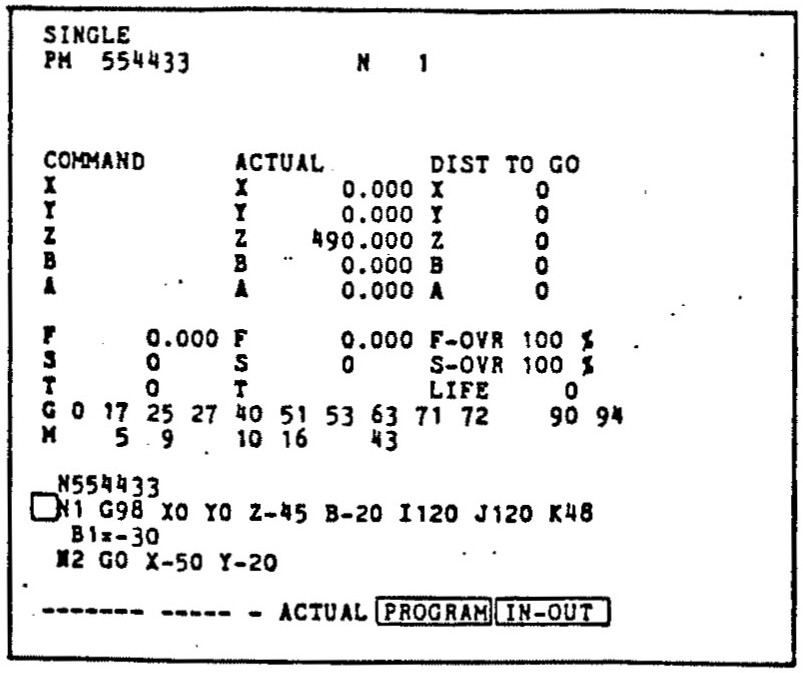
\includegraphics[width=0.6\textwidth]{program_execution.jpg}
\end{center}

After executing the current block, the block number \textbf{N} of the next block is displayed on \textbf{line 2} of the screen.

In the program section displayed on the screen, the cursor is positioned in front of the number of this block.

\begin{itemize}
    \iconitem{Press the \textbf{START} key again.}{start.jpg}
\end{itemize}

The procedure repeats.

At the end of the execution of the last block of the program, an automatic return to the start of the program occurs.  
The cursor is once again positioned on the program block number \textbf{N}.

\notes

It is possible to switch at any time from the \textbf{"program execution with individual block processing"} mode  
to the \textbf{"automatic program execution"} mode.

Pressing the \textbf{AUTO} key causes the \textbf{AUTO} signal to appear on \textbf{line 3} of the screen,  
indicating that automatic program execution has been selected. The current block is executed up to its end  
according to the previously used execution mode. After that, the machine stops.

Pressing the \textbf{START} key again restarts the machine and continues execution according to the automatic program mode.

In case of \textbf{error signals}, the procedure described in section \textbf{2.1} must be followed.

\newpage

\section{Automatic Program Execution (AUTO)}

In the \textbf{"automatic program execution"} mode, also known as \textbf{"AUTO"}, the part program is executed automatically until the \textbf{end of the program} or until a programmed stop.

\textbf{Programmed Stop}, see section \textbf{7.5}.

Automatic program execution can be interrupted at any time by pressing the stop key for feed motion or the stop key for the lead screw and spindle feed.

To resume an interrupted program execution, press the \textbf{START} key again.

\textbf{Feed rate adjustment:}  
The programmed feed rate can be adjusted within a range of \textbf{0 to 150\%},  
and the programmed rapid traverse rate can be modified within a range of \textbf{0 to 100\%} using intervention keys affecting the feed rate.

\textbf{Spindle speed adjustment:}  
The programmed spindle speed can be adjusted within a range of \textbf{80 to 120\%} in steps of \textbf{5\%} using the spindle speed correction keys.

\procedure

The program for machining the workpiece has been found using the procedure described in section \textbf{7.1.1}.

\begin{itemize}
    \iconitem{Press the \textbf{AUTO} key.}{auto.jpg}
\end{itemize}

The program number and the first blocks of the active program are displayed on \textbf{lines 19 to 22} of the screen.

\begin{itemize}
    \iconitem{Press the \textbf{START} key.}{start.jpg}
\end{itemize}

While the current block is being executed, its number \textbf{N} is displayed on \textbf{line 2} of the screen.

\begin{center}
    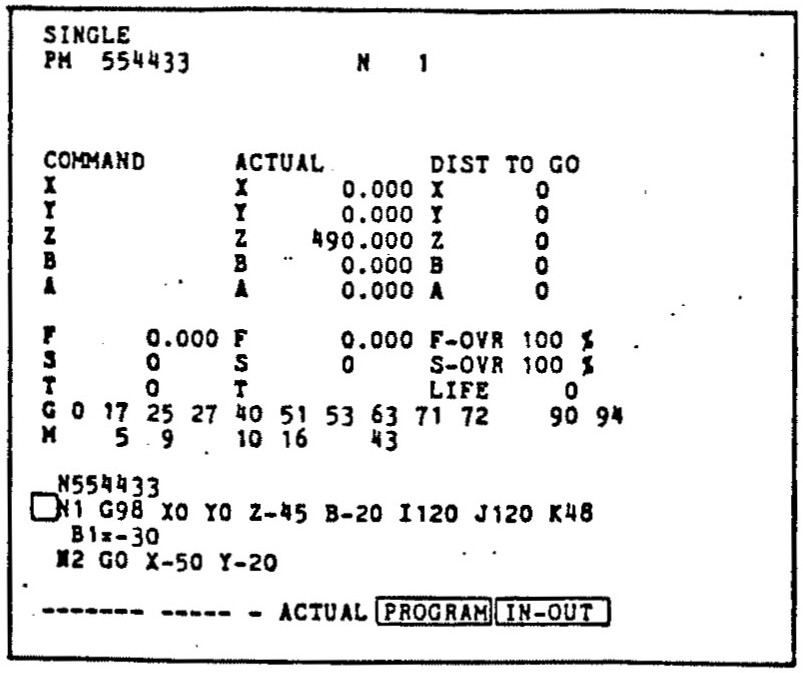
\includegraphics[width=0.7\textwidth]{program_execution.jpg}
\end{center}

After executing each block, the block number \textbf{N} of the next block appears on \textbf{line 2} of the screen.

In the displayed program section, the cursor always moves to the block number indicated on \textbf{line 2} of the screen.

After executing the \textbf{last} block of the program, an automatic return to the start of the program occurs.  
The cursor is once again positioned on the block number \textbf{N} of the program.

\notes

It is possible to switch at any time from the \textbf{"automatic program execution"} mode  
to the \textbf{"program execution with individual block processing"} mode.

Pressing the \textbf{SINGLE} key causes the \textbf{SINGLE} signal to appear on \textbf{line 3} of the screen,  
indicating that individual block processing mode has been selected.  
The current block is executed to completion according to the previously used execution mode.  
After that, the machine stops.

Pressing the \textbf{START} key again restarts the machine and continues execution  
according to the program with individual block processing.

In case of \textbf{error signals}, the procedure described in section \textbf{2.1} must be followed.

\section{Programmed Stop}

A block with a programmed stop (\textbf{M0}) is executed until completion.  
Executing this block interrupts the program.  
The feed drive mechanisms and the main drive system are deactivated.

The \textbf{M00} signal, displayed in an inverted manner, appears on \textbf{line 3} of the screen.

Program execution can be resumed at any time by pressing the \textbf{START} key.

The \textbf{M00} signal then disappears from \textbf{line 3} of the screen.
\newpage
\section{Manual Tool Change}

On machines \textbf{without an automatic tool changer}, when executing a block with a tool change instruction (\textbf{M6} or \textbf{M66}),  
program execution is interrupted so the tool can be changed \textbf{manually}.

The \textbf{INTERVENTION T} signal, followed by the tool number to be inserted into the spindle, appears on \textbf{line 3} of the screen (displayed in an inverted manner).

\begin{itemize}
    \iconitem{Press the \textbf{TOOL UNCL} key.}{tool_uncl.jpg}
\end{itemize}

Pressing this key automatically releases the tool.

The number of the tool to be removed from the spindle is displayed on \textbf{line 14} of the screen,  
to the right of the address letter \textbf{I}, shown in an inverted manner.

\begin{itemize}
    \item Manually remove the tool from the spindle.
    \item Insert the tool with the tool number \textbf{I} displayed on \textbf{line 2} of the screen.
\end{itemize}

\begin{itemize}
    \iconitem{Press the \textbf{TOOL UNCL} key.}{tool_uncl.jpg}
\end{itemize}

The automatic clamping device secures the tool,  
and the address letter \textbf{T} displayed on \textbf{line 14} of the screen \textbf{is no longer shown in inverted format}.

\begin{itemize}
    \iconitem{Press the \textbf{START} key.}{start.jpg}
\end{itemize}

The \textbf{INTERVENTION T} signal displayed on \textbf{line 3} of the screen disappears.

Program execution resumes.

The tool number \textbf{I} of the tool mounted in the spindle is now displayed on \textbf{line 14} of the screen.

\notes

For machines with an automatic tool changer, when executing a block with the tool change instruction \textbf{M6},  
no program interruption occurs. The tool is automatically changed after automatic retraction into the tool change position.

\newpage

\section{Program Interruption and Stop}

In \textbf{TEACH IN}, \textbf{SINGLE}, and \textbf{AUTO} operation modes,  
program execution can be interrupted and stopped at any time.

\subsection{Program Interruption}

\begin{itemize}
    \iconitem{Press the stop key for feed motion or the stop key for the lead screw and spindle feed.}{stop_feed.jpg, advance_stop_and_work_spindle.jpg}
\end{itemize}

The machine stops, and the program interruption is displayed on \textbf{line 3} of the screen by the \textbf{INTERVENTION} signal.

If it is necessary (e.g., for a control function) to move the axes in step mode:

\begin{itemize}
    \iconitem{Press the \textbf{MANUAL} key.}{manual.jpg}
\end{itemize}

The \textbf{MANUAL} signal displayed on \textbf{line 3} of the screen indicates that manual control has been selected.

The axes can now be moved in step mode.

If the interrupted program execution needs to be resumed:

\begin{itemize}
    \iconitem{Press the \textbf{TEACH IN}, \textbf{SINGLE}, or \textbf{AUTO} key, depending on the signal displayed on \textbf{line 1} of the screen (TEACH IN, SINGLE, or AUTO).}{teach_in.jpg, single.jpg, auto.jpg}
\end{itemize}

Pressing the corresponding key updates the screen to display the selected operation mode.

\begin{itemize}
    \iconitem{Press the \textbf{START} key.}{start.jpg}
\end{itemize}

The \textbf{INTERVENTION} signal disappears from \textbf{line 3} of the screen.

The axes first move automatically to the position that was reached at the time of program interruption.  
After this \textbf{repositioning}, program execution resumes.

\notes

Pressing the \textbf{MANUAL} key during program execution causes the \textbf{MANUAL} signal to appear on \textbf{line 3} of the screen,  
indicating that manual control has been selected.  
The current program block is executed to completion before the program is interrupted for manual operation.

An interrupted program can also be resumed by following the procedure described in \textbf{section 7.7.2}.

\subsection{Automatic Repositioning and Repetition of an Interrupted Block (REPOS)}

Resuming an interrupted program in \textbf{REPOS} mode first triggers automatic repositioning with linear docking to the position on the workpiece  
that was reached at the beginning of the interrupted block.  
Once repositioning is completed, the interrupted block is repeated \textbf{from the beginning of the block}.

The \textbf{REPOS} sub-mode is used when a block that has not yet been executed to completion  
must be repeated with a movement instruction without requiring prior modifications to the program.

\newpage

For example, if during the measurement of the workpiece a minimal excess thickness is detected on the contour,  
this excess thickness can be removed with a second pass by repeating the milling operation along the contour of the workpiece  
without modifying the program and simultaneously adjusting the programmed feed rate  
using the intervention keys that affect the feed rate or the programmed spindle speed  
using the intervention keys that affect the spindle rotation speed.

If necessary, a program modification can be made after the completion of the workpiece machining.

\procedure

The program was interrupted by pressing the stop key for feed movement  
or the stop key for the lead screw and the main spindle feed.

The program interruption is displayed by the \textbf{INTERVENTION} signal on \textbf{line 3} of the screen.

Before selecting the \textbf{REPOS} sub-mode, it may be necessary to take \textbf{precautionary measures}  
to \textbf{avoid collisions}, as the starting position of the interrupted block  
is \textbf{linearly approached} during automatic repositioning.

\begin{itemize}
    \iconitem{Press the \textbf{MENU} key.}{menu.jpg}
\end{itemize}

The program's sub-mode menu appears on the visualization screen:

\begin{center}
    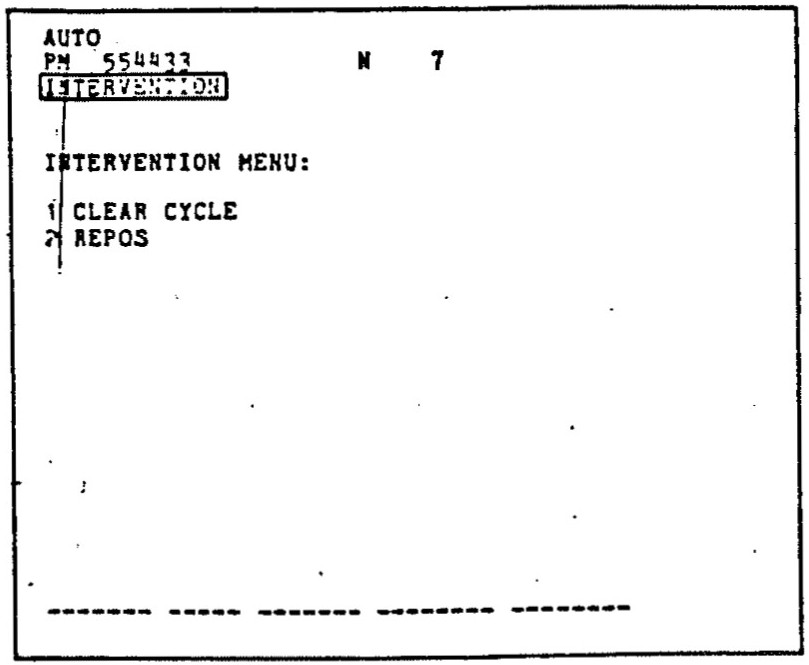
\includegraphics[width=0.7\textwidth]{intervention_menu.jpg}
\end{center}

\begin{itemize}
    \item Enter the digit \textbf{2} on the numeric keypad to select \textbf{REPOS}.
\end{itemize}

The \textbf{REPOS} signal, displayed in an inverted manner on \textbf{line 3} of the screen,  
indicates that the \textbf{REPOS} sub-mode has been selected.

\begin{itemize}
    \iconitem{Press the \textbf{START} key.}{start.jpg}
\end{itemize}

The \textbf{REPOS} signal disappears from \textbf{line 3} of the screen.

\newpage

\subsection{Stopping a Fixed Cycle (CLEAR CYCLE)}

In \textbf{TEACH IN}, \textbf{SINGLE}, and \textbf{AUTO} modes,  
a selected fixed cycle with function \textbf{G79} can be stopped at any time.

\procedure

\begin{itemize}
    \iconitem{Press the stop button for the feed movement or  
    the stop button for the lead screw and spindle feed.}{stop_feed.jpg, advance_stop_and_work_spindle.jpg}
\end{itemize}

The machine stops, and the fixed cycle interruption is displayed  
on \textbf{line 3} of the screen with the message \textbf{INTERVENTION CYCLE}.

\begin{itemize}
    \iconitem{Press the \textbf{MENU} button.}{menu.jpg}
\end{itemize}

The screen displays the menu of program sub-modes:

\begin{center}
    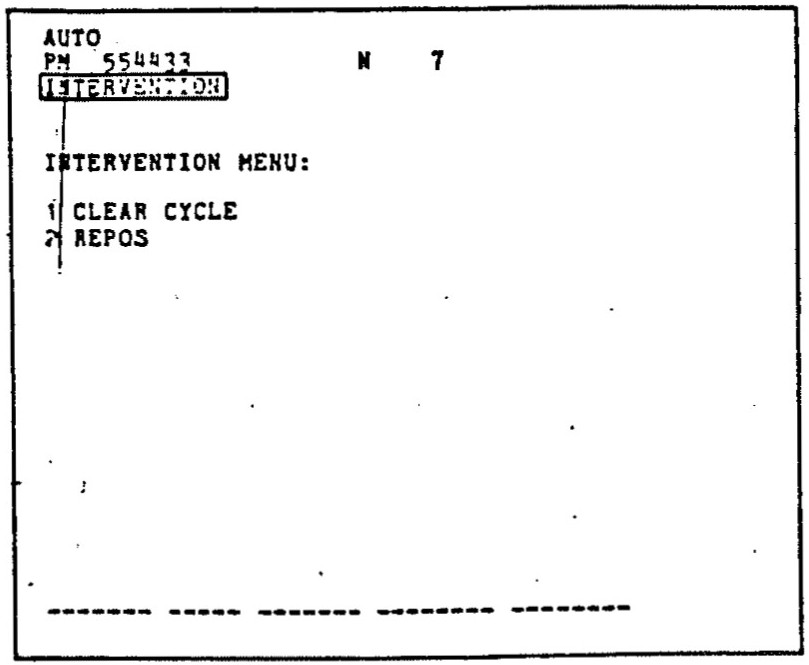
\includegraphics[width=0.7\textwidth]{intervention_menu.jpg}
\end{center}

\begin{itemize}
    \item Enter the number \textbf{1} on the numeric keypad to select \textbf{CLEAR CYCLE}.
\end{itemize}

The \textbf{CLEAR CYCLE} message, displayed on \textbf{line 3} of the screen,  
indicates that the interrupted fixed cycle must be canceled by pressing the \textbf{START} button.

\begin{itemize}
    \iconitem{Press the \textbf{START} button.}{start.jpg}
\end{itemize}

The cycle is stopped.

The tool is retracted to a position where it is above the workpiece surface,  
with the programmed safety distance.

After stopping the fixed cycle, modifications can be made within the program.

\textbf{Changing the Active Main Program}: See paragraph 6.2.

If the interrupted cycle needs to be \textbf{repeated}, it must be restarted in the program (see paragraph 7.1.1).

\notes

Stopping the tapping cycle G84 automatically changes the rotation direction, followed by the withdrawal of the tap to the safety distance.

\subsection{Stopping a Program}

\begin{itemize}
    \iconitem{Press the stop button for the feed movement or the stop button for the lead screw and working spindle feed.}{stop_feed.jpg, advance_stop_and_work_spindle.jpg}
\end{itemize}

The machine stops, and the program interruption is indicated by the display of the \textbf{INTERVENTION} signal on line 3 of the screen.

\notes

When \textbf{INTERVENTION CYCLE} is displayed, a tapping cycle G84 (according to paragraph 7.7.3) must be aborted before the \textbf{MANUAL} button can be activated.


\begin{itemize}
    \iconitem{Press the \textbf{MANUAL} button.}{manual.jpg}
\end{itemize}

After pressing the button, the axes can be moved step by step by manual positioning, if necessary.

\begin{itemize}
    \iconitem{Press the \textbf{CLEAR CONTR.} button.}{clear_contr.jpg}
\end{itemize}

Pressing this button resets the command to the \textbf{operating state}. In this case, an automatic start at the \textbf{beginning of the program} is performed.

\newpage

\section{E Parameter Table (EDIT PARAMETERS)}

The values of the \textbf{E} parameters used in the active machining program (see paragraph 3.6.1) are indicated in the \textbf{PARAMETERS} table and can be checked at any time during program execution.

However, these values are only \textbf{indicated} in this table \textbf{after execution} of the program blocks in which the parameters are defined or calculated with their values.

\procedure

\begin{itemize}
    \iconitem{Press the \textbf{PROG.MEM} button.}{prog_mem.jpg}
\end{itemize}
\vspace{.5cm}
\begin{itemize}
    \iconitem{Press the \textbf{MENU} button.}{menu.jpg}
\end{itemize}

On the display screen, the submenu for part programming appears:

\begin{center}
    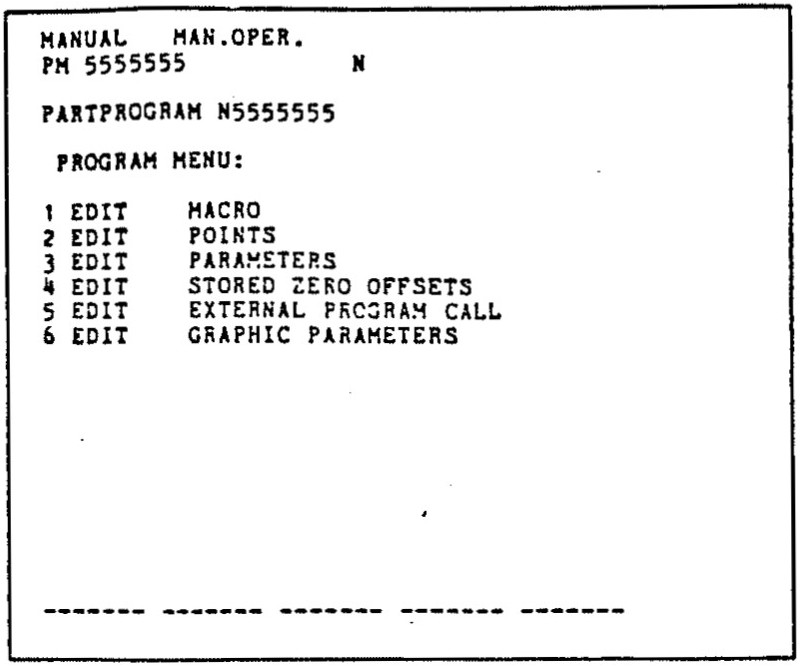
\includegraphics[width=0.8\linewidth]{program_menu.jpg}
\end{center}

\newpage

\begin{itemize}
    \item Enter the number \textbf{3} on the numeric keypad to select EDIT PARAMETER.
\end{itemize}

The parameter table appears on the screen:

\begin{center}
    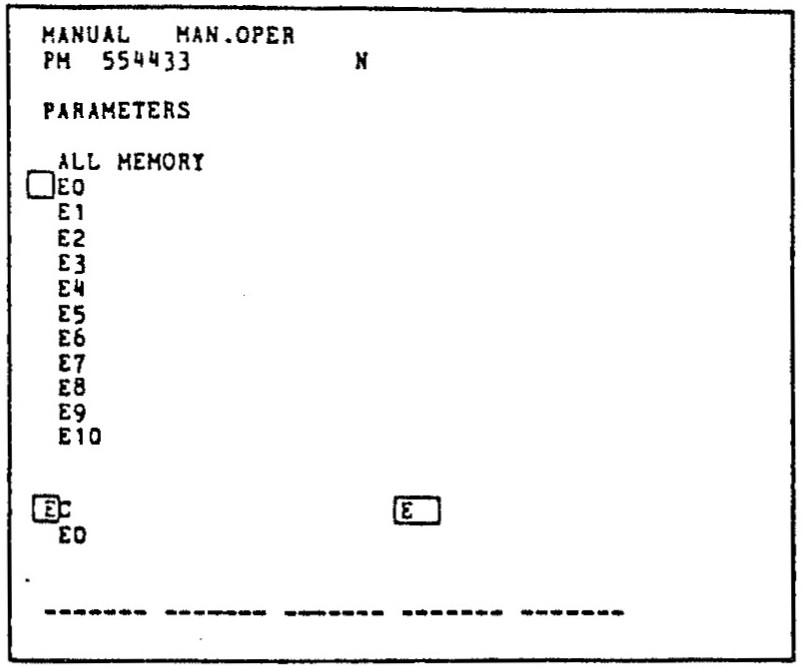
\includegraphics[width=0.8\linewidth]{parameter_table.jpg}
\end{center}

\begin{itemize}
    \iconitem{Move the cursor to the \textbf{E} parameter to be checked by pressing the up/down command buttons.}{up.jpg, down.jpg}
\end{itemize}

If one of the up/down command buttons is held down for more than one second, the cursor automatically jumps from one \textbf{P} parameter to the next.

If the desired \textbf{E} parameter is outside the visible section of the parameter table on the screen, it is \textbf{more useful} to search for it as follows:

\begin{itemize}
    \item Enter the number of the desired \textbf{E} parameter on the numeric keypad.
    \iconitem{Press the \textbf{ENTER} button.}{enter.jpg}
\end{itemize}
\vspace{.5cm}
\begin{itemize}
    \iconitem{Press the \textbf{SEARCH} button to start the search procedure.}{search.jpg}
\end{itemize}

After pressing the button, the cursor is placed in front of the located \textbf{E} parameter in the table.

\newpage

After checking the \textbf{E} parameters:

\begin{itemize}
    \iconitem{Press the \textbf{TEACH IN}, \textbf{SINGLE}, or \textbf{AUTO} button according to the signal displayed on line 1 of the screen (TEACH IN, SINGLE, or AUTO).}{teach_in.jpg, single.jpg, auto.jpg}
\end{itemize}

Pressing the corresponding button brings up the display for the relevant operating mode.

\notes

In \textbf{MANUAL} mode, parameter input is possible in the \textbf{EDIT PARAMETER} memory.

\section{Display Point Table (DISPLAY POINT)}

The coordinates assigned to the \textbf{P} points of the workpiece to be machined within the active machining program are indicated in the \textbf{PT} point table and can be checked at any time during program execution.

However, these coordinates are only \textbf{indicated} in this table \textbf{after execution} of the blocks in which the points are defined by their values.

\procedure

\begin{itemize}
    \iconitem{Press the \textbf{PROG.MEM} button.}{prog_mem.jpg}
\end{itemize}
\vspace{.5cm}
\begin{itemize}
    \iconitem{Press the \textbf{MENU} button.}{menu.jpg}
\end{itemize}

The submenu for machining programming appears on the screen:

\begin{center}
    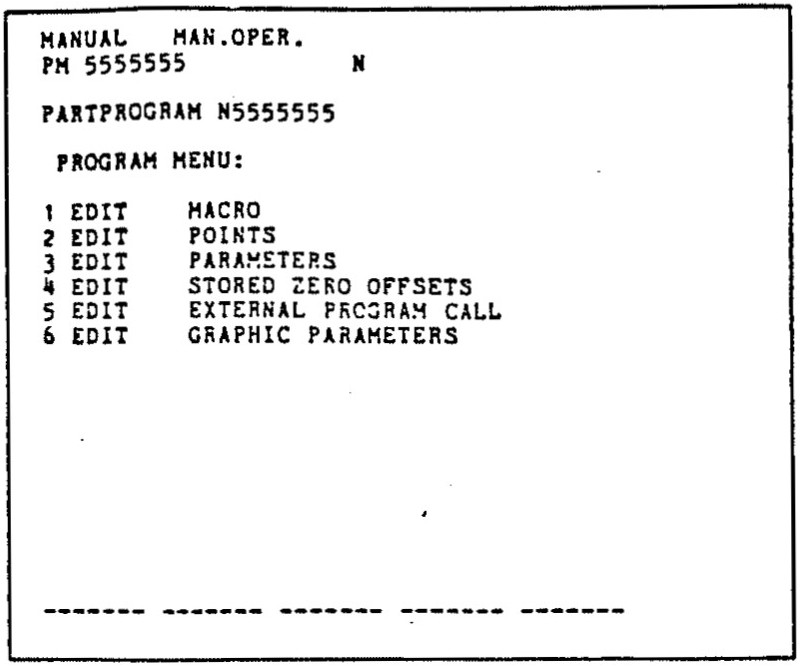
\includegraphics[width=0.6\linewidth]{program_menu.jpg}
\end{center}

\newpage
\begin{itemize}
    \item Enter the number \textbf{2} on the numeric keypad to select EDIT POINTS.
\end{itemize}

The point table appears on the screen:

\begin{center}
    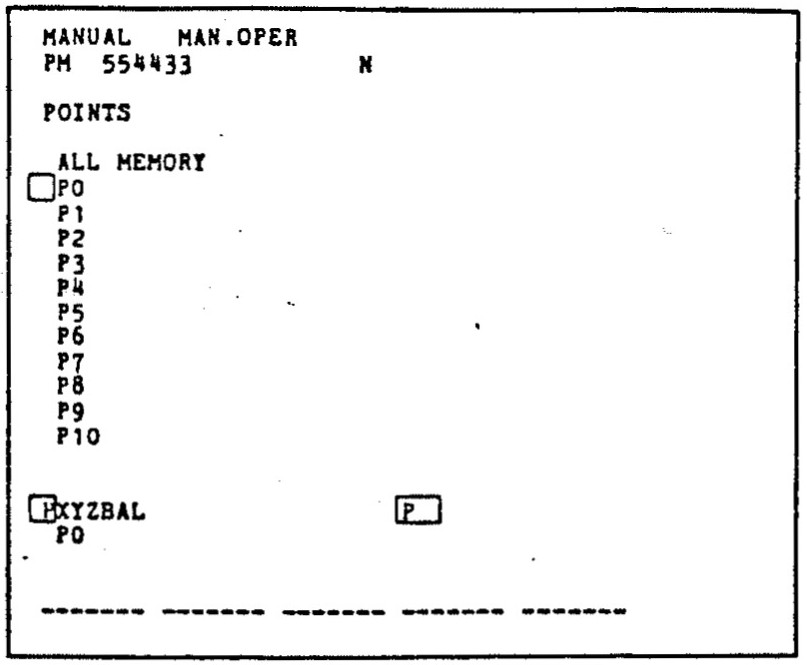
\includegraphics[width=0.6\linewidth]{point_table.jpg}
\end{center}

\begin{itemize}
    \iconitem{Move the cursor to the \textbf{P} point to be checked by pressing the up/down command buttons.}{up.jpg, down.jpg}
\end{itemize}

If one of the up/down command buttons is held down for more than one second, the cursor automatically moves from one \textbf{P} point to the next.

If the desired \textbf{P} point is outside the visible section of the \textbf{PT} point table on the screen, it is \textbf{more useful} to search for it as follows:

\begin{itemize}
    \item Enter the number of the desired \textbf{P} point on the numeric keypad.
    \iconitem{Press the \textbf{ENTER} button.}{enter.jpg}
\end{itemize}

\vspace{.5cm}

\begin{itemize}
    \iconitem{Press the \textbf{SEARCH} button to start the search procedure.}{search.jpg}
\end{itemize}

After pressing the button, the cursor is placed in front of the located \textbf{P} point in the \textbf{PT} point table.

After verifying the \textbf{P} points:

\begin{itemize}
    \iconitem{Press the \textbf{TEACH IN}, \textbf{SINGLE}, or \textbf{AUTO} button according to the signal displayed on line 1 of the screen (TEACH IN, SINGLE, or AUTO).}{teach_in.jpg, single.jpg, auto.jpg}
\end{itemize}

Pressing the corresponding button brings up the display for the relevant operating mode.

\notes

In \textbf{MANUAL} mode, points can be entered using the \textbf{EDIT POINTS} function.

\section{Shutting Down the Machine and Control System}

\begin{itemize}
    \iconitem{Press the \textbf{MANUAL} button.}{manual.jpg}
\end{itemize}

\vspace{.5cm}

\begin{itemize}
    \iconitem{Press the intervention button \textbf{"0\%"} affecting the feed rate.}{zero_percent.jpg}
    \item Press the red mushroom-shaped push button to shut down the hydraulic system and the machine's electrical system.
    \item Turn the main switch on the machine's electrical cabinet to \textbf{"Off"}.
\end{itemize}